% !TeX spellcheck = en_GB

\section{Requirements}\label{sec:requirements}

The following sections describe the primary requirements in the form of (quality) user stories.
Figure \ref{fig:requirements-overview} shows an overview of the primary use cases.

\begin{figure}[h]
    \centering
    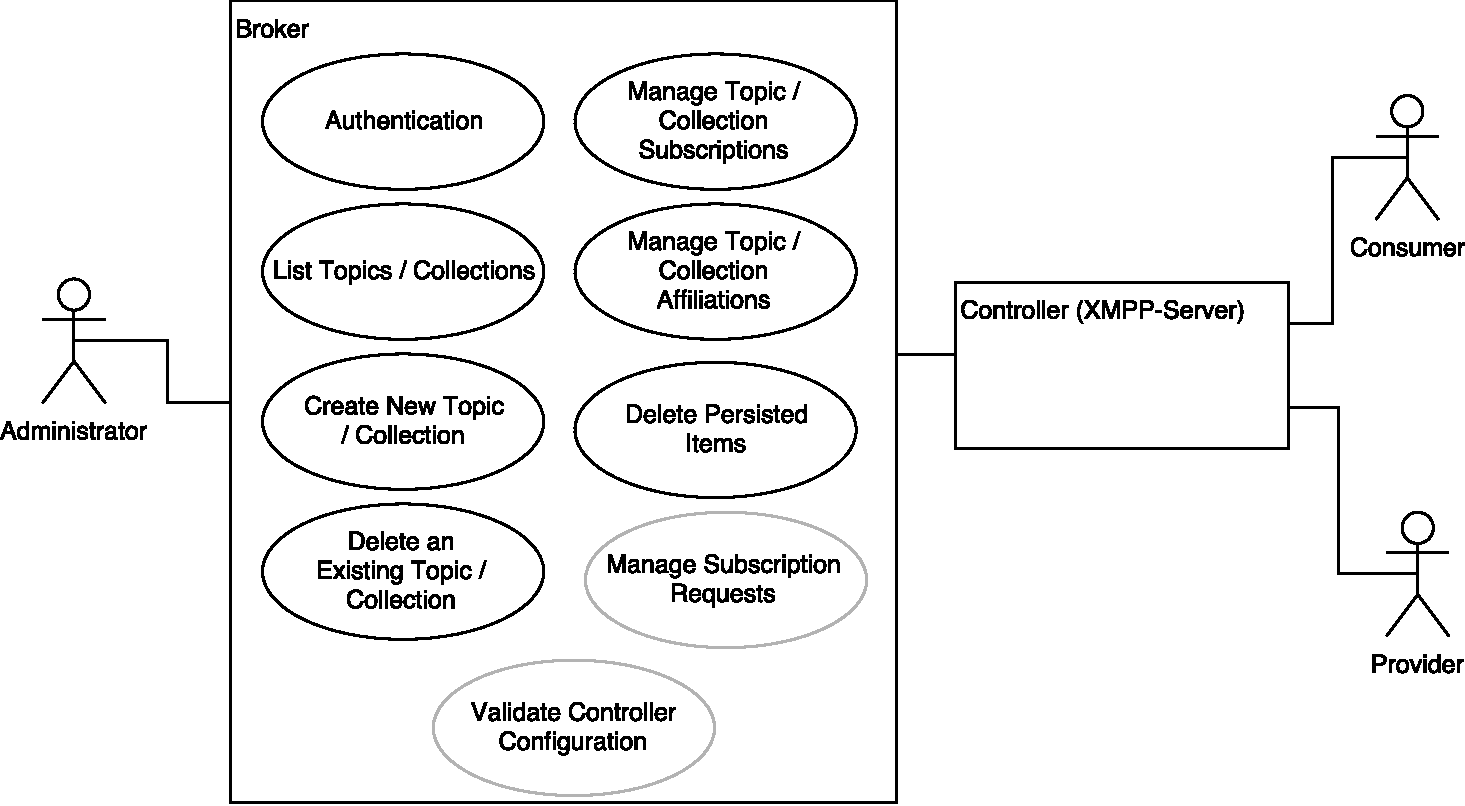
\includegraphics[width=1\linewidth]{resources/requirements_overview}
    \caption{UML Use Case Diagram presenting an overview of the primary component.}
    \label{fig:requirements-overview}
\end{figure}


% TODO: Search for more requirements in the ISO standard
% TODO: Spellcheck
% TODO: Vocabulary: Subscriber / Consumer

\subsection{01: Login}

As an Administrator,\\
I would like to log in\\
so that only I can inspect and manage topics.\\
To achieve this goal, I expect the following qualities (in descending order of priority):

\begin{itemize}
    \item The authentication time must on average not take 50\% longer than a regular XMPP-login from the client.
\end{itemize}

\noindent To be clarified:

\begin{itemize}
    \item It would be convenient to not maintain a separate user database and to use the same credentials for authentication
            as for the XMPP server and just forward them. This is from a security perspective usually not a great idea. Are there any
            specific requirements?
\end{itemize}

\subsection{01a: Secure XMPP Connection}

As an administrator concerned with security requirements,\\
I would like to use either SASL EXTERNAL or SASL SCRAM mechanism for authentication - \\
\begin{itemize}
    \item preferably the SCRAM-SHA-256-PLUS variant and
    \item preferably using mutual certificate-based authentication including revocation status checking
\end{itemize}

\noindent - so that the controller benefits from:

\begin{itemize}
    \item full accordance with the XMPP grid draft~\cite{ietf-mile-xmpp-grid-05}
    \item maximal security standards
\end{itemize}

\noindent To achieve this goal, I am willing to accept:
\begin{itemize}
    \item More costly and less user friendly authentication
    \item limited compatibility of supported XMPP servers
\end{itemize}

\subsection{02: Logout}

As an Administrator,\\
I would like to log out\\
to terminate a session.

\subsection{03: List available topics}

As an Administrator,\\
I would like to see a list of all topics on the controller\\
so that I can quickly assimilate \\
\begin{itemize}
    \item which topics exist
    \item if topics exist to which I have limited access for troubleshooting and debugging purposes
\end{itemize}

\subsection{04: Create a new topic}

As an Administrator,\\
I would like to create a new topic and optionally

\begin{itemize} % TODO: I guess these 2 should be smaller sub-stories...
    \item override the default configuration (eg. subscription model) 
    \item specify an initial set of consumers and providers
\end{itemize}

\subsection{05: Delete an existing topic}

As an Administrator,\\
I would like to delete an existing topic
to clean during development or get rid of obsolete topics.

To achieve this goal, I expect the following qualities (in descending order of priority):
\begin{itemize}
    \item prevent me from deleting the wrong topic (e.g. require me to enter the name of the topic manually)
\end{itemize}


\subsection{06: Manage topic subscriptions}

% TODO: Sub-Stories:
% 0. List all subscribed JIDs
% 1. show detailed subscription config
% 2. (partially) update the detailed subscription config
% 3. Unsubscribe subscribed JIDs
% 4. subscribe unsubscribed JIDs

\subsection{07: Manage topic affiliations}

% TODO: Sub-Stories:
% 1. ls all affiliated JIDs and their current role
% 2. Modify the role of the affiliated JIDs
%    (Allow to modify the JID of the admin - but warn me!)
% If we are not "owner" of a topic so, show a meaningful error message 

\subsection{08: Manage pending subscription requests}

As an Administrator,\\
I would like list pending subscription requests and approve or reject them\\
- given that this is feature supported by the target XMPP server -
to enable more dynamic access models than maintaining a blacklist and whitelist.

\subsection{09: Delete persisted Item in a Topic}

As an Administrator,\\
I would like to delete a specific persisted item in a topic\\
- given that this feature is supported by the target XMPP server -
to clean up test messages or remove obsolete or corrupt messages.

\subsection{10: Purge persisted Items in a Topic}

As an Administrator,\\
I would like to purge persisted items in a topic\\
- given that this feature is supported by the target XMPP server -
to clean up test messages or remove obsolete or corrupt messages.

\subsection{11: Validate controller configuration}

As an Administrator,\\
I would like to query the configuration and enabled extensions (XEPs) of the XMPP server\\
so that potential incompatibilities or suboptional configurations can simply be detected.

% \subsection{01: Login}

% As an Administrator,\\
% I would like to [goal]\\
% so that [effect (business value, impact)].\\
% To achieve this goal, I expect the following qualities (in descending order of priority):

% \begin{itemize}
%     \item measurable usability quality property, e.g. input steps required to complete story
%     \item measurable performance quality, e.g. average and worst case story response time
%     \item other verifiable quality goal if measurements are considered too risky/costly
% \end{itemize}


